\documentclass[a4paper,10pt]{article} 

\usepackage[utf8]{inputenc}     % UTF-8 Zeichensatz unter Linux -> ansonsten auf "applemac" oder "latin1" (Windows ISO-LANGE-NUMMER) ändern und diese Datei durch einen Konverter jagen ( Entsprechende Tools -> Google )


\usepackage[T1]{fontenc}        % Erweiterte Textcodierung (z.B a" -> ä)

\usepackage{textcomp}           % Extra Symbole (Grad Celsius etc.)
\usepackage{amssymb,amsmath}    % Schöne Formeln (AMS = American Mathematical Society)
\usepackage{graphicx}           % Bilder und Seitenränder
\usepackage{subcaption}			% captions for subfigures
\usepackage{booktabs}           % Schönere Tabellen
\usepackage{colortbl}           % Farbige Tabellen

%\usepackage[all]{hypcap}        % Verhaltenskorrektur für hyperref
%\usepackage{url}				% URLs
\usepackage{multirow}			% Tabellen mit mehreren Einträgen/Zeile
%\usepackage{tcolorbox}			% schöne bunte Boxen
\usepackage{mathtools}			% \mathclap für ordentliche \underbrace-			environments
\usepackage{geometry}			% Pagelayout mit \newgeometry, \restoregeometry
\usepackage{float}
\usepackage{wrapfig}
\usepackage{sidecap}			% side captions für Bilder; Befehl: % \begin{SCfigure}
\usepackage{bbm}				% for unity matrix (doublestroke 1) 
%\usepackage{pifont}
\usepackage{enumitem}
\usepackage{siunitx}			% proper SI unit typefacing
\usepackage{nicefrac}			% slanted fractions like 3/5
\usepackage{float}
\usepackage{braket}
%===============================%
\usepackage[singlelinecheck=false, figurename=Abb., aboveskip=7pt, belowskip=0pt]{caption}
				% richtet side captions ordentlich ein

%===============================%
%\bibliographystyle{dinat}       % Literaturverzeichnis nach DIN1505

% Change the itemize labels to some other symbol - needs enumitem
% where to look for graphics if they're not found
\graphicspath{{./img/}}



% bibliography style

\usepackage[numbers]{natbib} %use sort instead of cite
\bibliographystyle{unsrtnat}

\renewcommand{\k}{\mathbf{k}}
\begin{document}
\begin{titlepage}
 \begin{center}
	\Large{Advance laboratory class 2}
	\end{center}
	\begin{center}
	 \LARGE{\textbf{FP2 - Entanglement and Bell’s inequality}}
	\end{center}
	
	\begin{center}
	
	\large Marco \textsc{Canteri} \\
	marco.canteri@student.uibk.ac.at
	\end{center}
	
	\begin{center}
	\vspace{1cm}
	Innsbruck, \today
	\vspace{2cm}
	\end{center}
	
	\begin{center}
	\includegraphics[scale=0.4]{img/uibk} 
	\end{center}

\end{titlepage}
\begin{abstract}
In this work we performed correlation measurements on entangled photons produced by spontaneous parametric down conversion (SPDC). The purpose of this experiment was to test Bell's inequality
and thus check if quantum mechanics is complete or not. We found a Bell Parameter of $S = \pm$ which means that Bell's inequality doesn't hold.
\end{abstract}
\section{Introduction}
Historically quantum mechanics has been subjected of many critics due to its strange nature. Many attempts were made in order to explain this theory in a more intuitive way, one of these it the hidden variables interpretation of quantum mechanics. In order to test this interpretation Bell published an inequality \cite{bellpaper} that cannot be violated if the theory has hidden variable. The advantage of such inequality is that contains quantity that can be experimentally measured. This work it is a test of Bell's inequality, we used entangled photon in order to check this equality. Entangled photons are produced by SPDC inside a BBO ($\beta$ - BaB$_2$O$_4$) crystal. These photons are polarization entangled, this means that we can describe a state of two photons as, for example
\[\ket{\psi} = \frac{1}{\sqrt{2}}\left(\ket{HV} + \ket{VH}\right),\]
where $H$ and $V$ refer to horizontal and vertical polarization respectively. It is also possible to write the same state as a function of the $D/A$ basis, which correspond to $\pm 45$° polarization,
\[\ket{D} = \frac{1}{\sqrt{2}} \qquad \ket{A} = \frac{1}{\sqrt{2}}\]
(altra roba?).\\
There are different version of Bell's inequality, but for our experiment the most useful one was derived by Clauser, Horne, Shimony, and Holt [] and it is the following
\[S = |E(\alpha,\beta)-E(\alpha,\beta')|+|E(\alpha',\beta)+E(\alpha',\beta')|\leq 2,\]
where $S$ is called the Bell's parameter and $E(\alpha,\beta)$ is the expectation value of the polarization correlation measurements where the measure is made on a two photon system with the polarizers set at angle $\alpha$ and $\beta.$ In our experiment, this expectation value can be calculated with the number of coincidences as
\[E(\alpha,\beta) = \frac{1}{N}(C(\alpha,\beta)+C(\alpha+90,\beta+90)-C(\alpha+90,\beta)-C(\alpha,\beta+90)),\]
where $C(\alpha,\beta)$ is the number of coincidences with polarizer $A$ set to $\alpha$ and polarizer $B$ set to $\beta$ and $N$ is
\[N = (\alpha,\beta)+C(\alpha+90,\beta+90)+C(\alpha+90,\beta)+C(\alpha,\beta+90).\]


\section{Experiment setup}
\begin{figure}[H]
\centering
\includegraphics[width=\textwidth]{img/setup}
\caption{Schematic of the experiment setup}\label{setup}
\end{figure}
In figure \ref{setup} the experiment setup is depicted. We used a blue laser source of 404 nm and 100 mW of power. With help of some mirrors this light is focused into a BBO crystal where SPDC happens and entangled photons are created. This process is purely quantum mechanically, one pump photon is converted into a photon pair, a signal photon with vertical polarization and a idler photon with horizontal polarization. Energy conservation in this process must hold and can be written as
\[\hbar \nu_{pump} = \hbar \nu_{signal} + \hbar\nu_{idler},\]
this means that the sum of signal and idler frequencies must be equal to the frequency of the pump photon. Moreover, the photons must also obey momentum conservation which can is
\[\hbar \k_{pump} = \hbar \k_{signal} + \hbar\k_{idler}.\]
This implies that signal and idler photons are emitted in opposite direction with respect to pump photon, since wavevector must be conserved. Hence, entangled photons emerge in two different cones, and we can exploit this feature to split the beam in two separated different beams, one for the horizontal polarized photons and the other for the vertical polarized ones. This is done in the experiment setup using two small prisms. Then each photon goes through a lens that collimate the beam in a halfwave plate for rotating the polarization by 90 degrees and after inside another BBO crystal used to compensate walk off effects.  Walk off effects are due to the birefringence of the first

\section{Measurements and analysis}



\begin{thebibliography}{99}

  \bibitem{bellpaper}
     \textsc{J. Bell}, \textit{On the Einstein Podolsky Rosen paradox}, Physics, 1 (1964), pp. 195–200.

  \bibitem{Zmass}
   J. Beringer et al. (Particle Data Group), PR D86, 010001 (2012)

   \bibitem{Zdecay}
   http://pdg.lbl.gov/2009/tables/rpp2009-sum-gauge-higgs-bosons.pdf

   \bibitem{ratio}
   The ATLAS Collaboration JHEP 1012(2010)060

   \bibitem{Zchannel}
   http://pdg.lbl.gov/2012/listings/rpp2012-list-z-boson.pdf
   \bibitem{Wchannel}
	http://pdg.lbl.gov/2012/listings/rpp2012-list-w-boson.pdf
\end{thebibliography}
\end{document}
